\documentclass[a4paper]{article}
\usepackage[text={165mm,245mm}]{geometry}
\usepackage{graphicx}
\usepackage{subfigure}
\usepackage{ctex}
\usepackage{float} 
\usepackage{amsmath}
\usepackage{listings}
\usepackage{xcolor}
\definecolor{mygreen}{rgb}{0,0.6,0}  
\definecolor{mygray}{rgb}{0.5,0.5,0.5}  
\definecolor{mymauve}{rgb}{0.58,0,0.82}  
  
\lstset{ %  
  backgroundcolor=\color{white},   % choose the background color; you must add \usepackage{color} or \usepackage{xcolor}  
  basicstyle=\footnotesize,        % the size of the fonts that are used for the code  
  breakatwhitespace=false,         % sets if automatic breaks should only happen at whitespace  
  breaklines=true,                 % sets automatic line breaking  
  captionpos=bl,                    % sets the caption-position to bottom  
  commentstyle=\color{mygreen},    % comment style  
  deletekeywords={...},            % if you want to delete keywords from the given language  
  escapeinside={\%*}{*)},          % if you want to add LaTeX within your code  
  extendedchars=true,              % lets you use non-ASCII characters; for 8-bits encodings only, does not work with UTF-8  
  frame=single,                    % adds a frame around the code  
  keepspaces=true,                 % keeps spaces in text, useful for keeping indentation of code (possibly needs columns=flexible)  
  keywordstyle=\color{blue},       % keyword style  
  %language=Bin,                 % the language of the code  
  morekeywords={*,...},            % if you want to add more keywords to the set  
  numbers=left,                    % where to put the line-numbers; possible values are (none, left, right)  
  numbersep=5pt,                   % how far the line-numbers are from the code  
  numberstyle=\tiny\color{mygray}, % the style that is used for the line-numbers  
  rulecolor=\color{black},         % if not set, the frame-color may be changed on line-breaks within not-black text (e.g. comments (green here))  
  showspaces=false,                % show spaces everywhere adding particular underscores; it overrides 'showstringspaces'  
  showstringspaces=false,          % underline spaces within strings only  
  showtabs=true,                  % show tabs within strings adding particular underscores  
  stepnumber=1,                    % the step between two line-numbers. If it's 1, each line will be numbered  
  stringstyle=\color{orange},     % string literal style  
  tabsize=2,                       % sets default tabsize to 2 spaces  
  %title=myPython.py                   % show the filename of files included with \lstinputlisting; also try caption instead of title  
}  
\title{\heiti 
CODH - 运算器及其应用 \hspace{0.3cm}实验报告}
\author{院系: \kaishu\underline{}\hspace{1.5cm}姓名: \kaishu \underline{}\hspace{1.5cm}学号: \kaishu \underline{}\hspace{1.5cm}}
\begin{document}
\maketitle

\section{实验目的}
\begin{itemize}
    \item 熟练掌握算术逻辑单元 (ALU) 的功能
    \item 掌握数据通路和控制器的设计方法
    \item 掌握组合电路和时序电路,以及参数化和结构化的Verilog描述方法
    \item 了解查看电路性能和资源使用情况
\end{itemize}

\section{实验环境}
\begin{itemize}
  \item vlab.ustc.edu.cn
  \item Vivado 2016.3
  \item Nexys 4 DDR 开发板
\end{itemize}
\section{实验内容}
\subsection{实现算术逻辑单元 (ALU) }
\begin{itemize}
  \item f:功能选择,加、减、与、或、异或、逻辑左移、逻辑右移、算术右移等运算
  \item a, b:两个操作数
  \item y:运算结果,和、差 …… 
  \item t:比较标志,相等(eq),小于(lt, ltu)
\end{itemize}

\subsection{ALU的应用:计算移动/滑动平均 (MAV)}
\begin{itemize}
  \item d:输入数据
  \item en:输入使能
  \item m:输出数据
  \item clk, rstn:时钟,复位信号
\end{itemize}

\section{逻辑设计 / 核心代码}
\subsection{算术逻辑单元 (ALU) }
\subsubsection{逻辑设计}
只需要使用Verilog基本运算以及组合逻辑即可实现,注意\texttt{f=3'b000} (减法计算)时需要对\texttt{t}进行特殊计算
。
(相等时\texttt{t[0] = 1},无符号小于时\texttt{t[2] = 1},有符号小于时\texttt{t[1] = 1})。

\subsubsection{核心代码}
\begin{lstlisting}[language={verilog},title={alu.v}] 
  always @ (*)
  begin
    t = 3'b000;
    case(f)
    3'b000: 
    //t[0] = 1 if a eq b
    //t[1] = 1 if a < b (signed)
    //t[2] = 1 if a < b (unsigned)
    begin
        y = a - b; 
        if(y == 0)
            t[0] = 1;
        if(a < b)
            t[2] = 1;
        if($signed(a) < $signed(b))
            t[1] = 1;
    end
    3'b001: y = a + b;
    3'b010: y = a & b;
    3'b011: y = a | b;
    3'b100: y = a ^ b;
    3'b101: y = a >> b;
    3'b110: y = a << b;
    3'b111: y = $signed(a) >>> b; 
    endcase
  end
\end{lstlisting}

\subsubsection{模块仿真}
直接对默认的32位 ALU 进行仿真,使用系统的 \texttt{\$random} 函数生成随机的 a 和 b,对每一种 f 进行仿真。 
testbench 如下:
\begin{lstlisting}[language={verilog},title={alu.v}] 
  ...
  alu alu_inst(a, b, s, y, f);
  initial 
  begin
      a = $random;
      b = $random;
      s = 0;
  end

  initial
  begin
      for(i=0; i<8; i=i+1)
      begin
          #5 s = s + 1;
      end
  $finish;
  end
\end{lstlisting}
在 Vivado 仿真后得到波形图:
\begin{figure}[H]
  \centering
  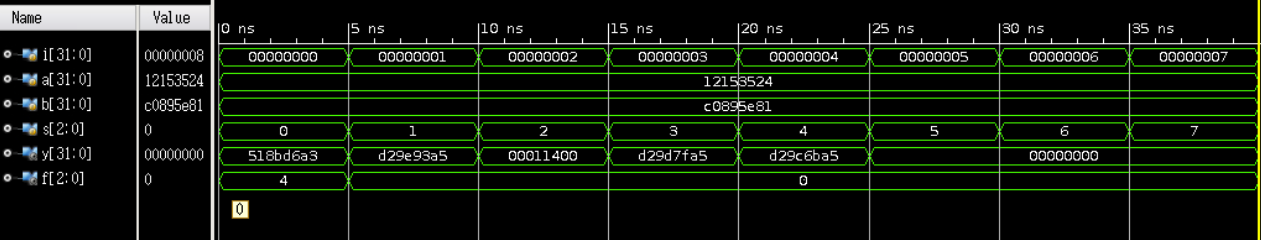
\includegraphics[width=1.0\textwidth]{alu_sim.png}
  \caption{ALU仿真波形图}
  \label{fig:alu}
\end{figure}

注意到最后有关移位的部分,因为b过大导致结果都为0,实际上正确性没有问题。如果可以对b进行限制(取模),可能结果会更加直观。
\subsubsection{下载测试}
由于一开始无法烧写板子,故首先在FPGAOL平台上进行了调试,之后
编写 alu\_top 进行测试,将 ALU 的输入输出接到开发板上,使用开发板上的按键和 LED 来进行 ALU 的输入和输出,结果与设计相符合。因为仅仅是一个组合逻辑电路,没有加入时钟,因此没有时间性能报告。

RTL电路图:
\begin{figure}[H]
  \centering
  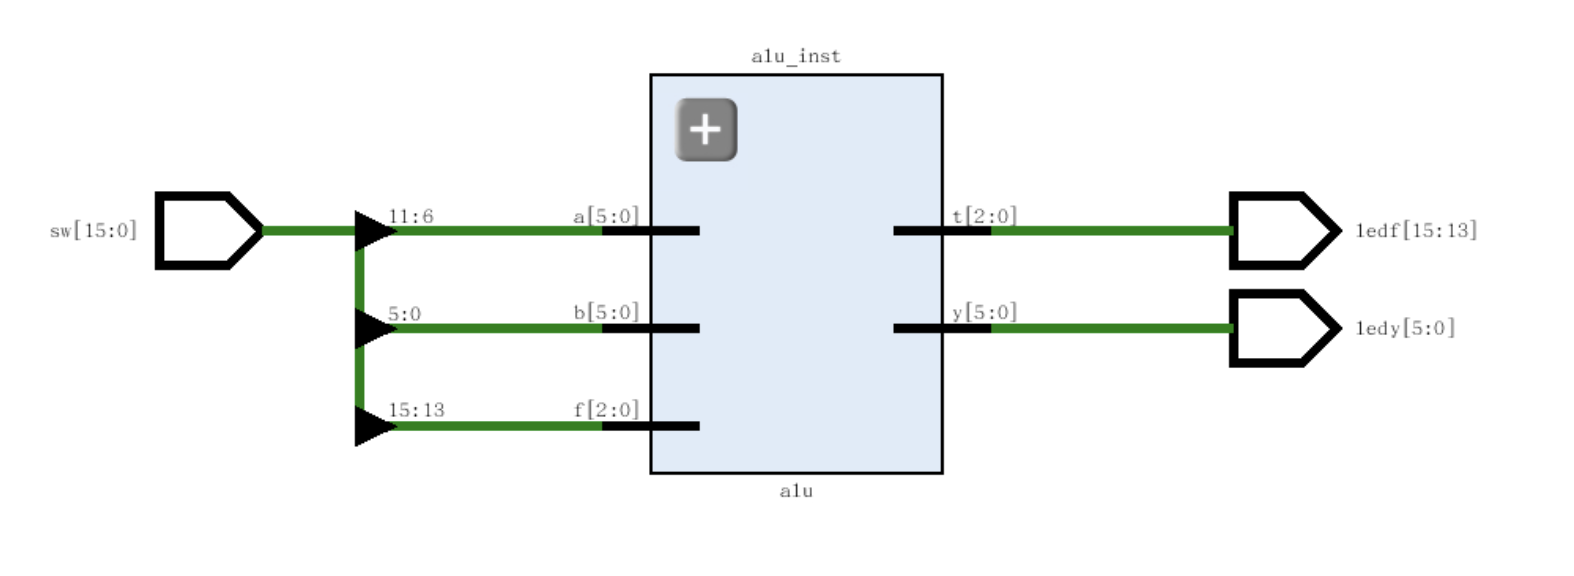
\includegraphics[width=1.0\textwidth]{alu_rtl.png}
  \caption{ALU RTL电路图}
  \label{fig:alu_rtl}
\end{figure}

电路资源使用情况:
\begin{figure}[H]
  \centering
  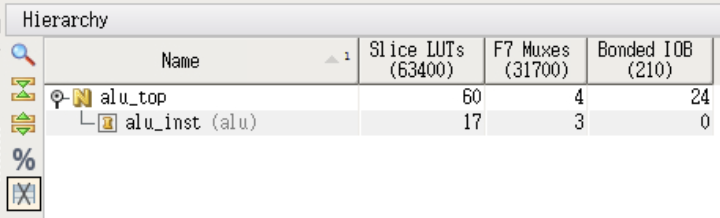
\includegraphics[width=1.0\textwidth]{alu_cir.png}
  \caption{ALU 电路资源使用情况}
  \label{fig:alu_rtl}
\end{figure}

\subsection{计算移动/滑动平均 (MAV) }
\subsubsection{逻辑设计}
状态机方面,共设计五个状态,需要3位二进制码表示:未输入数字(IDLE)、已输入一个数字(M1)、已输入两个数字(M2)、已输入三个数字(M3)、已输入四个数字(M4)。
使用四个寄存器(m0、m1、m2、m3)来存储之前输入的四个数字。

初始状态记为IDLE,此时初始化m0、m1、m2、m3为0,输出数据(m)为0。

对于每个状态,当时针上升沿到来时,如果使能信号(EN)为1,则将寄存器内容向后移动,将输入数据(d)存入第一个寄存器(m0);如果使能信号为0,则不改变数据寄存器。

对于前四个状态,输出数据(m)为之前的输入数据(d),当时针上升沿到来时,如果使能信号为1,则切换至下一个状态,否则保持当前状态。

最后一个状态输出的是对四个寄存器内数据的平均值,借用ALU,可以实现累计,并且可以通过向右位移2位来实现除以4的效果。

状态转换图如下:

\begin{figure}[H]
  \centering
  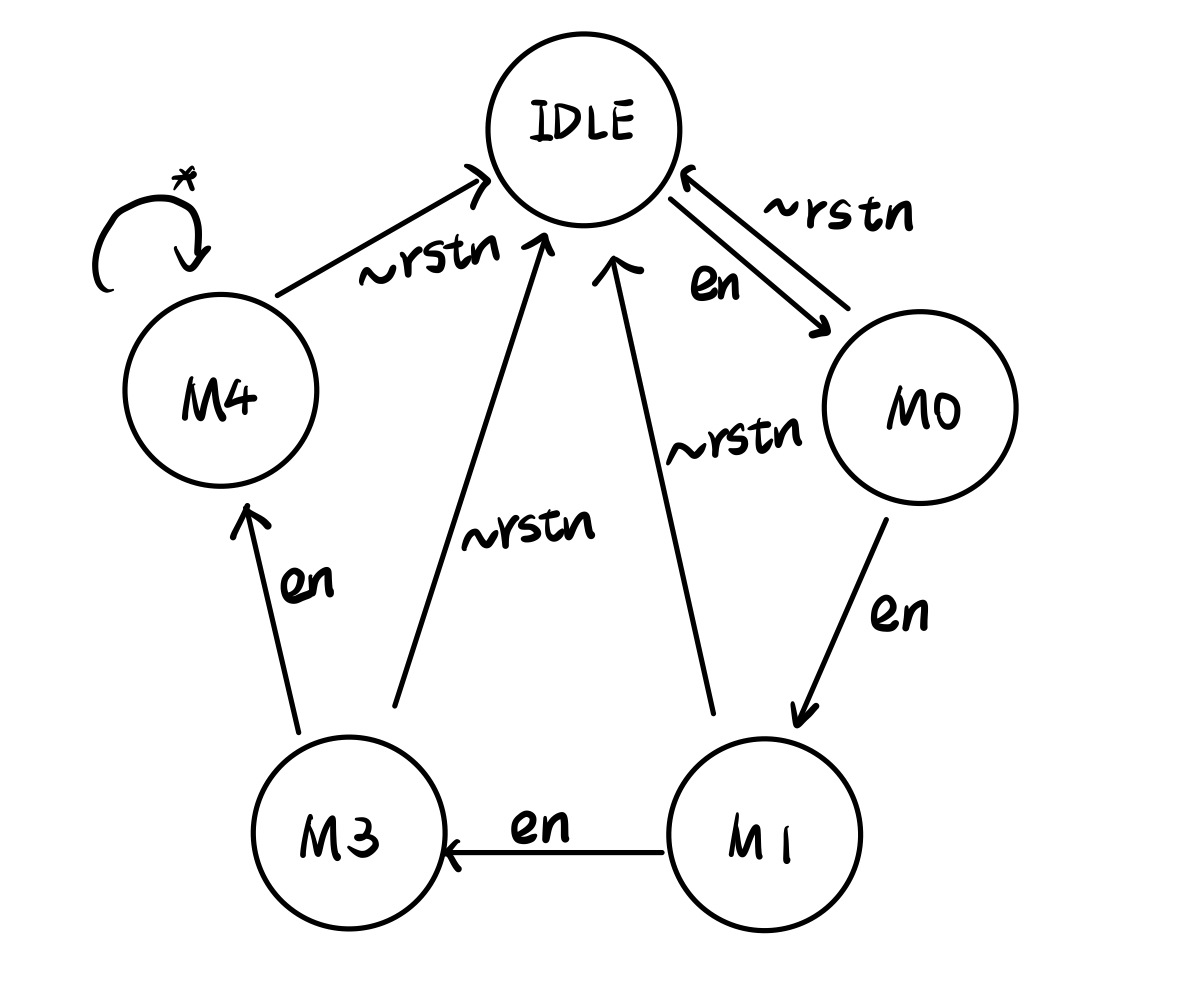
\includegraphics[width=0.5\textwidth]{mav_graph.jpeg}
  \caption{MAV状态转换图}
  \label{fig:mav_g}
\end{figure}
\subsubsection{核心代码}
\begin{lstlisting}[language={verilog},title={mav.v}]
    ...
    //三段式状态机
    //此处四个例化ALU用于计算(m0+m1+m2+m3)/4
    alu #(.WIDTH(16)) alu_inst1(d, m0, 3'b001, temp1);
    alu #(.WIDTH(16)) alu_inst2(m1, m2, 3'b001, temp2);
    alu #(.WIDTH(16)) alu_inst3(temp1, temp2, 3'b001, temp3);
    alu #(.WIDTH(16)) alu_inst4(temp3, 16'o2, 3'b111, res);
    //状态切换
    always@(posedge clk or negedge rstn) begin
        if(~rstn)
            cs <= 3'b000;
        else
            cs <= ns;
    end
    //决定次态
    always@(*) begin
        ns = cs;
        if(en) begin
            case(cs)
                IDLE: begin ns = M1; end
                M1: begin ns = M2; end
                M2: begin ns = M3; end
                M3: begin ns = M4; end
                M4: begin ns = M4; end
                default begin ns = IDLE; end
        endcase
        end
    end
    //输出部分
    always@(posedge clk or negedge rstn) begin
        if(~rstn) begin
                m0 <= 16'b0;
                m1 <= 16'b0;
                m2 <= 16'b0;
                m3 <= 16'b0;
                m <= 16'b0;
        end
        else if(en) begin
            m0 <= d;
            m1 <= m0;
            m2 <= m1;
            m3 <= m2;
            if(ns == 3'b100) begin
                m <= res;
            end
            else
                m <= d;
        end
    end
\end{lstlisting}
\subsubsection{模块仿真} 
对照老师提供的波形图编写 testbench:
\begin{lstlisting}[language={verilog},title={mav.v}]
  ...
  mav mav_inst(clk, rstn, en, d, m);

  initial 
  begin
      rstn = 0;
      #7 rstn = ~rstn;
  end

  initial
  begin
      clk = 0;
      forever
          #5 clk = ~clk;
          #5 clk = ~clk;
          en = ~en;
  end
  initial
      begin
          en = 0;
          forever
              #10 en = ~en;
      end
  initial
  begin
      d = 31'o2;
      #20 d = 31'o3;
      #20 d = 31'o4;
      #20 d = 31'o5;
      #20 d = 31'o6;
      #30 $finish;
  end
\end{lstlisting}
在Vivado进行仿真,波形图如下:
\begin{figure}[H]
  \centering
  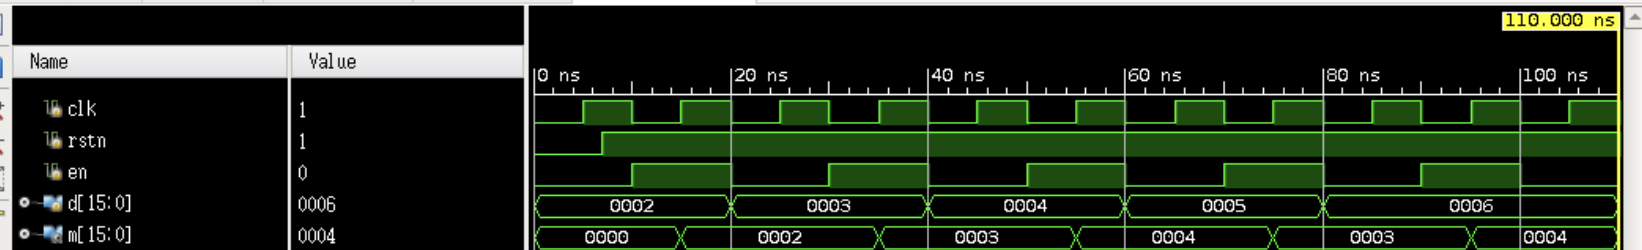
\includegraphics[width=1.0\textwidth]{mav_sim.png}
  \caption{MAV仿真波形图}
  \label{fig:mav}
\end{figure}
可以发现MAV模块很好地完成了任务。
\subsubsection{下载测试}
首先需要编写取边沿,去抖动的模块,对en进行处理:
\begin{lstlisting}[language={verilog},title={edge.v}]
  ...
  always@(posedge clk)
    begin
        if (en == 0)
            cnt <= 0;
        else if (cnt < 16'h8000)
            cnt <= cnt + 1;
        en1 <= cnt[15];
        en2 <= en1;
    end
  assign out = en1 & ~en2;
\end{lstlisting}
然后编写mav\_top模块,同时为了更直观的看到结果,除了用16位LED作为输出之外还添加了4位7短管来显示4位16进制的输出。
这里实例化mav模块,使用了edge模块来处理使能信号,encode模块来将输出数据m的每四位转化为7段管的显示码,使用了分时轮流显示4位7段管来达到同时显示的效果。
\begin{lstlisting}[language={verilog},title={mav\_top.v}]
  module mav_top (
    input  clk, 
    input  rstn, 
    input  en,
    input  [15:0]  d,
    output [15:0]  m,
    output [7:0] AN,
    output CA, CB, CC, CD, CE, CF, CG
);
    wire out;
    integer t = 0;
    reg [7:0] in_temp, AN_temp;
    fix_edge edge_inst1(clk, en, out);
    mav mav_inst1(clk, rstn, out, d, m);

    encode encode_inst(
        .in(in_temp),
        .out1(CA),
        .out2(CB),
        .out3(CC),
        .out4(CD),
        .out5(CE),
        .out6(CF),
        .out7(CG)
    );
    
    always @ (posedge clk)
    begin
        if(t % 100000 == 0)
        begin
            t = 0;
            case(AN_temp)
                8'b11111110: begin AN_temp = 8'b11111101; in_temp = m[7:4]; end
                8'b11111101: begin AN_temp = 8'b11111011; in_temp = m[11:8]; end
                8'b11111011: begin AN_temp = 8'b11110111; in_temp = m[15:12]; end
                default: begin AN_temp = 8'b11111110; in_temp = m[3:0]; end
           endcase
        end
        t = t + 1;
    end
    assign AN = AN_temp;
endmodule
\end{lstlisting}
七段管编码显示,encode模块:
\begin{lstlisting}[language={verilog}, title={encode.v}]
    ...  
    case (in)
        4'b0000: begin out = 7'b1000000; end
        4'b0001: begin out = 7'b1111001; end
        4'b0010: begin out = 7'b0100100; end
        4'b0011: begin out = 7'b0110000; end
        4'b0100: begin out = 7'b0011001; end
        4'b0101: begin out = 7'b0010010; end
        4'b0110: begin out = 7'b0000010; end
        4'b0111: begin out = 7'b1111000; end
        4'b1000: begin out = 7'b0000000; end
        4'b1001: begin out = 7'b0010000; end
        4'b1010: begin out = 7'b0001000; end
        4'b1011: begin out = 7'b0000011; end
        4'b1100: begin out = 7'b1000110; end
        4'b1101: begin out = 7'b0100001; end
        4'b1110: begin out = 7'b0000110; end
        4'b1111: begin out = 7'b0001110; end
        default: begin out = 7'b1111111; end
        endcase
    end
    assign {out7, out6, out5, out4, out3, out2, out1} = {out};
    ...
\end{lstlisting}
然后生成bit流进行测试。由于笔记本不兼容,一开始先在FPGAOL平台上对简化版的mav\_top进行了测试,测试结果一切正常。

之后再烧写到Nexys 4 DDR上进行测试,测试结果与预期相符,已供助教检查。助教同时指出了一些可以简化的部分,因此检查结束后又改进了部分代码(相较于检查时添加了7段数码管显示、简化了状态机的转换)。

\subsubsection{结果分析}
RTL电路:寄存器转换级电路,根据硬件寄存器之间的数字信号(数据)流以及对这些信号执行的逻辑操作来模拟同步数字电路。
\begin{figure}[H]
  \centering
  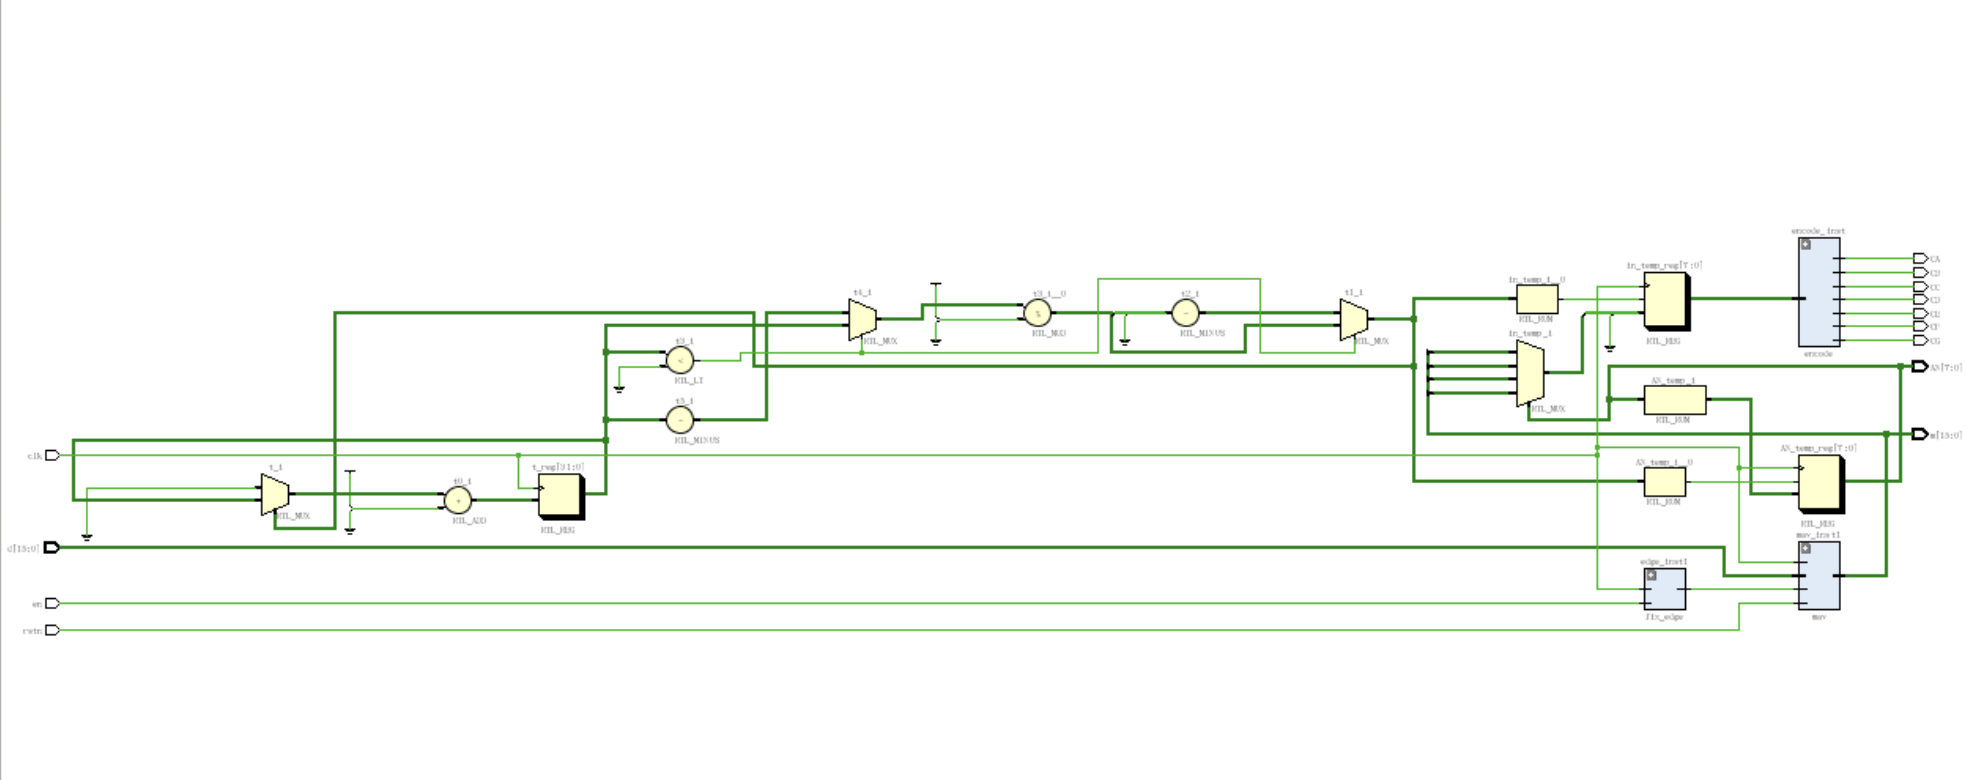
\includegraphics[width=1.0\textwidth]{rtl.png}
  \caption{RTL电路图}
  \label{fig:mav_rtl}
\end{figure}
可以发现由于mav\_top对7段数码管输出的支持使得RTL电路图变得很复杂,删去这一部分后再查看:
\begin{figure}[H]
  \centering
  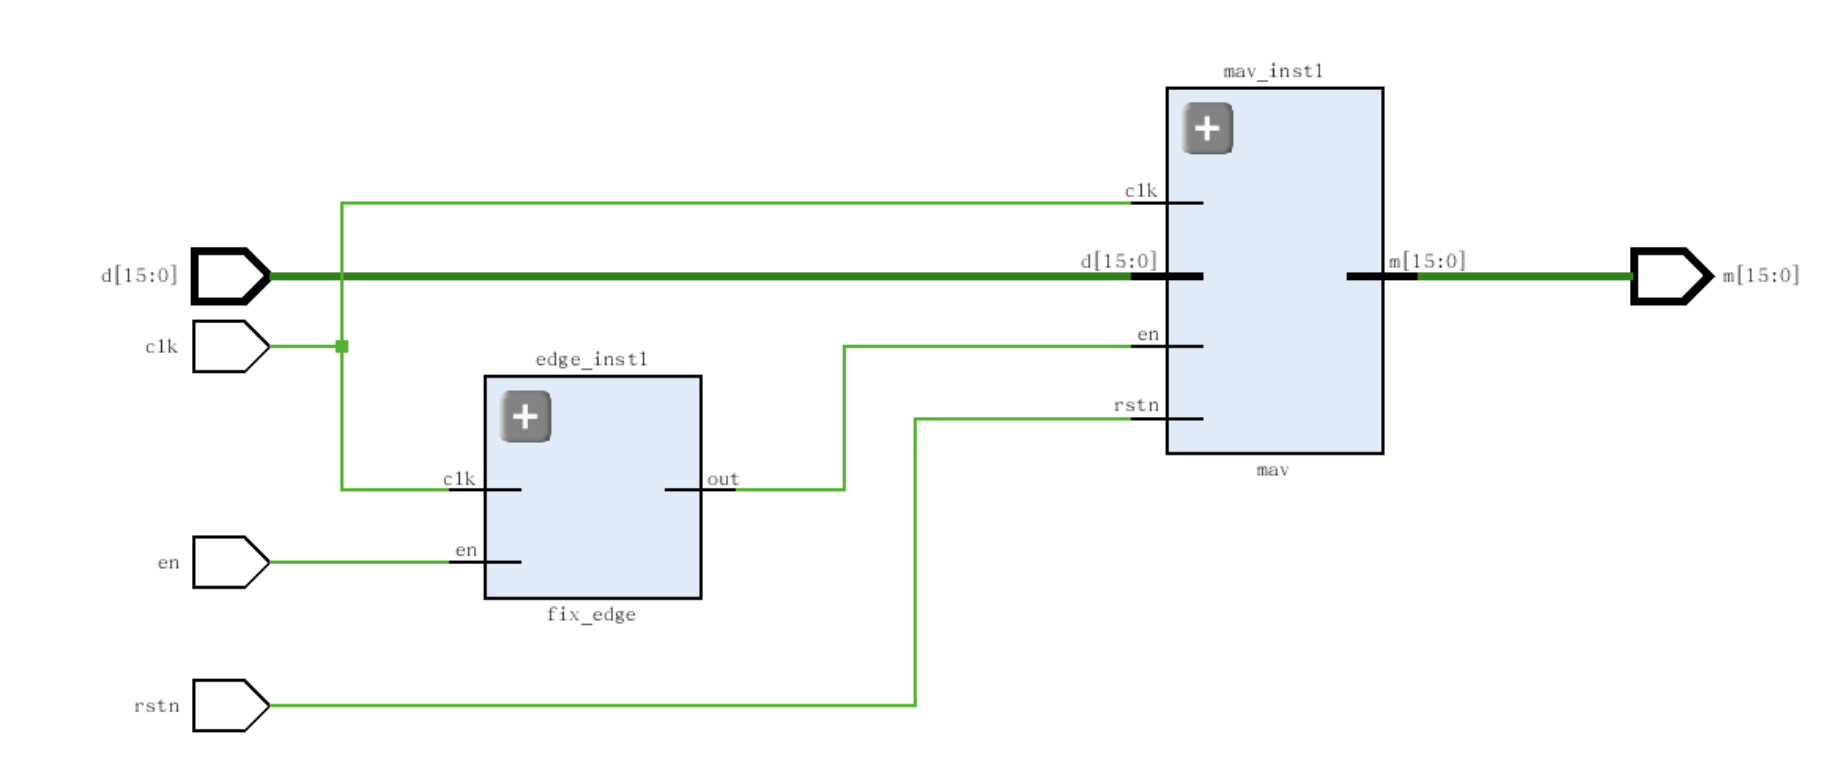
\includegraphics[width=1.0\textwidth]{rtl_1.png}
  \caption{RTL电路图}
  \label{fig:mav_rtl_1}
\end{figure}

电路资源使用情况:
\begin{figure}[H]
  \centering
  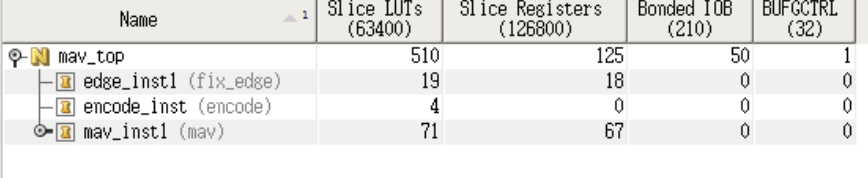
\includegraphics[width=1.0\textwidth]{mav_cir.png}
  \caption{电路资源使用情况}
  \label{fig:mav_cir}
\end{figure}
时间性能报告:
\begin{figure}[H]
  \centering
  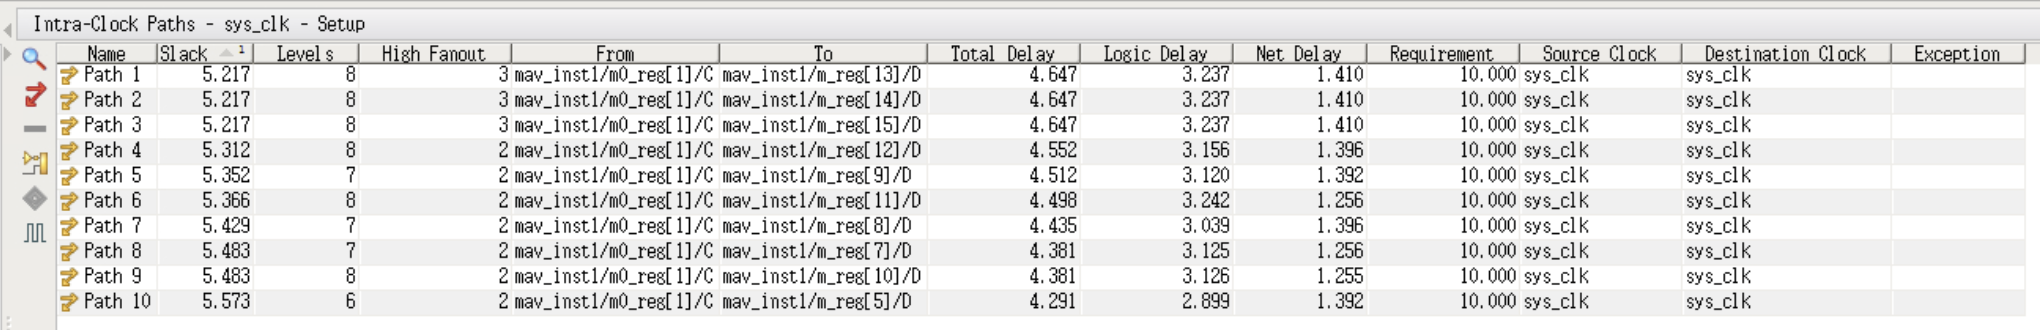
\includegraphics[width=1.0\textwidth]{mav_time.png}
  \caption{时间性能报告}
  \label{fig:mav_time}
\end{figure}
\section {结果分析}
每个 Xilinx 7 系列 FPGA的Slice 包含4个 LUT 查找表 和8个触发器,还可以包含寄存器、进位链和多个多数选择器。

关于电路资源使用情况:这里前两列显示的就是模块占用的 LUT 以及 Register 的数目;Bonded IOB指占用的可编程输入输出单元数目,BUFGCTRL指占用的时钟缓冲器数目。

关于时间性能报告:Timing Summary报告把路径按照时钟域(例如Intra-Clock,同一时钟域内部路径)分类,每个组别下缺省会报告Setup、Hold以及Pulse Width检查最差的各10条路径,其中一些参数意义如下:
\begin{enumerate}
  \item slack:建立时间裕量
  \item level:逻辑级数,这里1就表示在两个寄存器之间仅存在1个组合逻辑器件
  \item fanout:表示从这一点连接到了几个目的端点,fanout = 1就表示连接了1个目的端点
  \item from to:表示是哪两者之间的时序
  \item logic delay:逻辑器件延时
  \item net delay:布线延时
\end{enumerate}
\section {实验总结}
\begin{enumerate}
  \item 本次实验尽管在开始时由于我的硬件条件不支持对烧录程序造成了一些麻烦,但依然很好地锻炼了我设计状态图,从底向上分模块构建代码完成试验任务的能力;同时也磨练了调试代码的技术。
  \item 加深了对开发板的理解,意识到了仿真的重要性;完善的仿真模拟可以减少很多的硬件调试,效率会高上不少。
  \item 学会了更好地设计状态机,在助教的指导下检查出状态间重复可以合并的部分,使得代码更加简洁。
  \item 了解到了如何使用7段数码管显示数字,使得输出更加直观。
  \item 学会了查看RTL电路,电路资源使用情况,时间性能报告等。并且通过搜索引擎了解到了这些后续分析的意义所在。
\end{enumerate}
\section {意见/建议}
如果可能的话,建议增加实验室开放时间。由于硬件条件不兼容,第一次实验可能耗费了许多时间在无用的尝试之上,如果平时也能够在实验室进行实验,那么效率会高上不少。
\end{document}